\section{Definisi}

Arsitektur komputer adalah suatu konsep perencanaan dan juga struktur pengoperasian dasar dari suatu sistem komputer atau ilmu yang bertujuan untuk perancangan sistem komputer. Arsitektur komputer dapat dikategorikan sebagai ilmu sekaligus sebuah seni mengenai cara interkoneksi antara berbagai komponen perangkat keras atau hardware untuk dapat menciptakan sebuah komputer yang dapat memenuhi kebutuhan fungsional, kinerja, dan juga target biaya dalam bidang teknik komputer. 

Arsitektur  von Neumann (atau Mesin Von Neumann) adalah arsitektur yang diciptakan oleh John von Neumann [1903 – 1957]. Arsitektur ini digunakan oleh hampir pada semua komputer pada saat ini. Arsitektur Von Neumann ini menggambarkan komputer dengan 4 (empat) bagian utama, yaitu: Unit Aritmatika dan Logis (ALU), unit kontrol, memori, dan alat masukan dan hasil (secara kolektif dinamakan I atau O). Bagian tersebut dihubungkan oleh berkas kawat, “bus”. 

Arsitektur komputer merupakan suatu hal yang sangatlah penting karena dapat memberikan berbagai atribut-atribut pada sistem komputer, hal tersebuti tentunya sangat dibutuhkan bagi perancang ataupun user software sistem dalam mengembangkan suatu program.

Arsitektur komputer memiliki 2 bagian utama yaitu:
\begin{itemize}
\item Instructure Set Architecture
Instructure Set Architecture (ISA) adalah spesifikasi yang menentukan bagaimana programmer bahasa mesin berinteraksi dengan komputer.
\item Hardware System Architecture
Hardware Set Architecture (HSA) adalah subsistem hardware (perangkat keras) dasar yaitu CPU, Memori, serta OS.

\end{itemize}


\section{Sejarah}

Awal mula komputer yang sebenarnya dibentuk oleh seoarng profesor matematika Inggris, Charles
Babbage (1791-1871). Tahun 1812, Babbage memperhatikan kesesuaian alam antara mesin
mekanik dan matematika:mesin mekanik sangat baik dalam mengerjakan tugas yang sama
berulangkali tanpa kesalahan; sedang matematika membutuhkan repetisi sederhana dari suatu
langkah-langkah tertenu. Masalah tersebut kemudain berkembang hingga menempatkan mesin
mekanik sebagai alat untuk menjawab kebutuhan mekanik. Usaha Babbage yang pertama untuk
menjawab masalah ini muncul pada tahun 1822 ketika ia mengusulkan suatu mesin untuk melakukan
perhitungan persamaan differensil. Mesin tersebut dinamakan Mesin Differensial. Dengan
menggunakan tenaga uap, mesin tersebut dapat menyimpan program dan dapat melakukan kalkulasi serta mencetak hasilnya secara otomatis. Setelah bekerja dengan Mesin Differensial selama sepuluh
tahun, Babbage tiba-tiba terinspirasi untuk memulai membuat komputer general-purpose yang
pertama, yang disebut Analytical Engine. Asisten Babbage, Augusta Ada King (1815-1842)
memiliki peran penting dalam pembuatan mesin ini. Ia membantu merevisi rencana, mencari
pendanaan dari pemerintah Inggris, dan mengkomunikasikan spesifikasi Anlytical Engine kepada
publik. Selain itu, pemahaman Augusta yang baik tentang mesin ini memungkinkannya membuat
instruksi untuk dimasukkan ke dlam mesin dan juga membuatnya menjadi programmer wanita yang
pertama. Pada tahun 1980, Departemen Pertahanan Amerika Serikat menamakan sebuah bahasa
pemrograman dengan nama ADA sebagai penghormatan kepadanya.

Mesin uap Babbage, walaupun tidak pernah selesai dikerjakan, tampak sangat primitif apabila
dibandingkan dengan standar masa kini. Bagaimanapun juga, alat tersebut menggambarkan elemen
dasar dari sebuah komputer modern dan juga mengungkapkan sebuah konsep penting. Terdiri dari
sekitar 50.000 komponen, desain dasar dari Analytical Engine menggunakan kartu-kartu perforasi
(berlubang-lubang) yang berisi instruksi operasi bagi mesin tersebut \cite{sudirman2003sejarah}.

\begin{enumerate}
\item Generaasi Pertama (1945 - 1955)

Negara-negara maju yang sedang berperang berlomba-lomba menciptakan peralatan canggih yang digunakan untuk media informasi dan radar  untuk keperluan militer. Komputer diperkenalkan pertama kali di universitas Pensylvania dengan berbasis teknologi tabung hampa udara  yang digunakan pada peralatan radio. Konsep utama arsitektur komputer diperkenalkan oleh john Von Neuman,
Program dan datanya diletakkan dalam memori yang sama , operasi aritmatika dasar dilakukan dalam beberapa milidetik menggunakan teknologi tabung hampa udara untuk menerapkan fungsi logika, teknologi ini dapat menghasilkan peningkatan kecepatan  dengan kelipatan 100 hingga 1000 kali relatif terhadap teknologi mekanik dan elektro mekanik berbasis relay dan  fungsi I/O dilaksanakan oleh alat yang mirip mesin ketik.

\item Generasai kedua (1955-1965)

Perusahan AT\&T Bell laboratories menemukan Transistor pada akhir tahun 1940-an dan dengan cepat menggantikan tabung hampa udara, pada  periode ini dikembangkan memori berinti magnetic, bahasa tingkat tinggi, program system yang disebut Compiler, Prosedure I/O terpisah juga dikembangkan. Pada periode ini IBM menjadi produsen komputer terbesar.

\item Generasi ketiga (1965-1975)

Dengan ditemukannya  IC ( Integrated circuit) mulai menggantikan memori berinti magnetic, adanya pengenalan microprogramming, pararelism, software system operasi memungkinkan pembagian yang efisien suatu system komputer oleh beberapa program user (multiuser), selain itu dikembangkan memori cache virtual, computer  mainframe system 360 dari IBM dan jenis mini komputer PDP dari Digital Equipment Corporation merupakan komersial yang dominan pada generasi ini

\item Generasi keempat (1975 – sekarang)

Teknik Fabrikasi Integreted circuit berevolusi  ketitik derah processor utama lengkap dengan pembagian besar dari memori utama suatu komputer kecil yang dapat diimplementasikan pada chip tunggal dengan 10000 transistor.generasi ini terus berkembang dengan ditemukannya Very large scale integration (VLSI) sehingga memungkinkan processor berkembang semakin cepat.dan kemampuan memori mencapai kecepatan 2n. 


\end{enumerate}



\section{Software dan Hardware}
\subsection {Software}

Pengertian Software komputer adalah sekumpulan data elektronik yang disimpan dan diatur oleh komputer, data elektronik yang disimpan oleh komputer itu dapat berupa program atau instruksi yang akan menjalankan suatu perintah. Melalui sofware atau perangkat lunak inilah suatu komputer dapat menjalankan suatu perintah. ( contoh software \ref{fig:software})

\begin{figure}[!htbp]
  \centering
  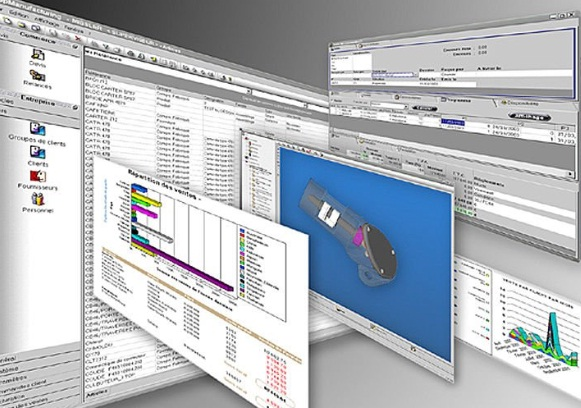
\includegraphics[width=.75\textwidth]{figures/software/software.jpg}
  \caption{Ini adalah contoh software}\label{fig:software}
\end{figure}


\subsubsection{Perngertian Software Menurut Para Ahli}

\begin{enumerate}
\item Menurut Wiwit Siswoutomo, software adalah nyawa dari sebuah hardware atau komputer karena tanpa adanya perangkat lunak maka komputer hanyalah sebuah hardware yang mati dan tidak dapat digunakan.

\item Menurut Roger S. Pressman (2002), pengertian software adalah suatu perintah program dalam sebuah komputer yang apabila dieksekusi oleh usernya akan memberikan fungsi dan unjuk kerja seperti yang diharapkan oleh user-nya. Dengan kata lain, perangkat lunak berfungsi untuk memberi perintah kepada komputer agar dapat berfungsi secara optimal sesuai dengan perintah user.

\item Menurut Melwin Syafrizal Daulay (2007), pengertian software adalah suatu perangkat yang berfungsi sebagai pengatur aktivitas kerja komputer dan seluruh intruksi yang mengarah pada sistem komputer dan menjembatani interaksi antara user dengan komputer.

\item Menurut Imam Prayogo Pujiono, pengertian perangkat lunak adalah suatu program dalam komputer yang dirancang sedemikian rupa, yang jika dijalankan akan memberikan perintah ke komputer/ hardware/ software lain dalam rangka menyelesaikan sebuah tugas, pekerjaan, dan juga tuntutan tertentu seperti yang diharapkan user.

\item Menurut Wilman dan Riyan, pengertian software adalah sebuah perangkat operasi kerja untuk menjalankan berbagai komponen pada hardware yang memiliki sifat maya (tidak terlihat) tetapi bermanfaat bagi user-nya.
\end{enumerate}

\subsubsection{Fungsi Software}

Pada dasarnya fungsi utama software adalah untuk membuat sebuah komputer dapat menjalankan perintah dari user. Mengacu pada pengertian software yang dijelaskan di atas, adapun beberapa fungsi software adalah sebagai berikut:

\begin{enumerate}
\item Menyediakan fungsi dasar dari sebuah komputer sehingga dapat dioperasikan. Misalnya ketersediaan sistem operasi dan sistem pendukung pada komputer.

\item Mengatur setiap hardware yang ada pada komputer sehingga dapat bekerja secara simultan.

\item Menjadi penghubung antara beberapa perangkat lunak lainnya dengan hardware yang ada pada komputer.

\item Perangkat lunak juga berfungsi sebagai penerjemah suatu perintah software lainnya ke dalam bahasa mesin, sehingga dapat dimengerti oleh hardware.

\item Software juga dapat mengidentifikasi suatu program yang ada pada sebuah komputer.
\end{enumerate}

\subsubsection{Software Berdasarkan Jenisnya}

\begin{itemize}

\item Operating System (sistem operasi), yaitu perangkat lunak yang berfungsi untuk mengelola dan mengkoordinasikan setiap komponen dan fungsi komputer. Beberapa contoh operating sistem adalah; Windows, Linux, UNIX, DOS.

\item Programming Language (Bahasa Pemrograman), yaitu perangkat lunak yang berfungsi sebagai pemberi instruksi standar yang melibatkan sintak dan semantik yang dipakai untuk mendefinisikan suatu program aplikasi komputer (computer application program). Beberapa contoh Bahasa Pemrograman adalah; PHP, Java, Microsoft Visual Basic.

\item Application Program (Program Aplikasi), yaitu perangkat lunak yang memiliki fungsi tertentu, misalnya software untuk presentasi, software akuntansi, dan lain sebagainya. Beberapa contoh Program Aplikasi adalah; Microsoft Office Word, Microsoft Office Excel, MYOB, OpenOffice.org, dan lainnya.
\end{itemize}

\subsubsection{Software Berdasarkan Distribusinya}

\begin{itemize}
\item Freeware, yaitu perangkat lunak yang dapat dimiliki dan digunakan secara gratis tanpa batas waktu tertentu. Biasanya perangkat lunak jenis ini memiliki fitur yang kurang lengkap dan tidak maksimal.

\item Adware, yaitu software yang bisa didapatkan dan digunakan secara gratis namun dengan kompensasi adanya iklan yang muncul di komputer user.

\item Spyware, yaitu perangkat lunak yang dibuat khusus untuk memata-matai segala aktivitas pengguna komputer. Biasanya software jenis ini banyak disalahgunakan, misalnya untuk mencuri data dari komputer lain.

\item OpenSource, yaitu software yang kode sumbernya dapat dibuka, diubah-ubah, ditingkatkan, dan disebarluaskan. Biasanya software jesni ini dapat diperoleh secara gratis dan dapat dikembangkan oleh orang lain dengan lisensi GPL (General Public License).

\item Shareware, yaitu piranti lunak untuk keperluan tertentu yang dibagikan secara gratis, biasanya sebagai demonstrasi dengan fitur terbatas dan penggunaannya untuk waktu terbatas (misalnya 30 hari).

\end{itemize}

\subsection{Hardware}

Perangkat keras komputer adalah semua bagian fisik komputer, dan dibedakan dengan data yang berada di dalamnya atau yang beroperasi di dalamnya, dan dibedakan dengan perangkat lunak (software) yang menyediakan instruksi untuk perangkat keras dalam menyelesaikan tugasnya.

Hardware dalam bahasa Indonesia disebut juga dengan nama “perangkat keras” yaitu salah satu komponen dari sebuah komputer yang sifat alatnya bisa dilihat dan diraba secara langsung atau yang berbentuk nyata, yang berfungsi untuk mendukung proses komputerisasi. Hardware dapat bekerja berdasarkan perintah yang telah ditentukan atau disebut juga dengan istilah “instruction set”. Adanya perintah yang dapat dimengerti oleh hardware, maka hardware tersebut dapat melakukan berbagai kegiatan yang telah ditentukan oleh pemberi perintah.

Secara fisik, Komputer terdiri dari beberapa komponen yang merupakan suatu sistem. Sistem adalah komponen-komponen yang saling bekerja sama membentuk suatu kesatuan. Apabila salah satu komponen tidak berfungsi, akan mengakibatkan tidak berfungsinya proses-proses yang ada pada komputer dengan baik. Komponen komputer ini termasuk dalam kategori elemen perangkat keras (hardware). Berdasarkan fungsinya, perangkat keras komputer dibagi menjadi 3 :

\begin{enumerate}

\item Input Device (unit masukan)

Unit ini berfungsi sebagai media untuk memasukkan data dari luar ke dalam suatu memori dan processor untuk diolah guna menghasilkan informasi yang diperlukan. Data yang dimasukkan ke dalam sistem komputer dapat berbentuk signal input dan maintenance input. Signal input berbentuk data yang dimasukkan ke dalam sistem komputer. Sedangkan maintenance input berbentuk program yang digunakan untuk mengolah data yang dimasukkan.

Jadi, Input device selain digunakan untuk memasukkan data dapat pula digunakan untuk memasukkan program. Berdasarkan sifatnya, peralatan input dapat digolongkan menjadi 2 yaitu :

\begin{itemize}
\item Peratalan input langsung, yaitu input yang dimasukkan langsung diproses oleh alat pemroses. Contohnya : keyboard, mouse, touch screen, light pen, digitizer graphics tablet, scanner.

\item Peralatan input tidak langsung, input yang melalui media tertentu sebelum suatu input diproses oleh alat pemroses. Contohnya : punched card, disket, harddisk.
\end{itemize}

\item Process Device (Unit Pemrosesan)

Perangkat pengolah data dipergunakan untuk mengolah data. Pengolah data meliputi unit pengolah pusat (CPU/Central Processing Unit) dan juga mikroprosesor. CPU (Central Processing Unit) merupakan alat yang berfungsi sebagai pemroses data. CPU berisi rangkaian sirkuit yang menyimpan instruksi-instruksi pemrosesan dan penyimpanan data.

Beberapa sirkuit tersebut terdapat Motherboard, Processor, Memory (RAM), Kartu Grafis (VGA Card), Kartu Suara (Sound Card), Harddisk, Floopy Disk Drive, DVD Room, Power Supply, Baterai CMOS, Fan, Heatsink, dll. 

Unit pemrosesan yang berada dalam komputer adalah Central Processing Unit (CPU). CPU merupakan otak atau pengatur suatu sistem yang mengolah sehingga menghasilkan informasi. 

Ada tiga unsur penting yang ada dalam CPU :

\begin{itemize}
\item Primary storage adalah ukuran besarnya processor atau biasa disebut dengan main memory.
\item Arithmatic logic unit adalah suatu alat yang bertugas melakukan perhitungan dalam komputer
\item Control unit adalah merupakan suatu alat pengontrolan yang berada dalam komputer yang memberitahukan unit masukan mengenai jenis data, waktu pemasukan, dan tempat penyimpanan didalam primary storage. Control unit juga bertugasmemberitahukan kepada arthmaticlogic unit mengenai operasi yang harus dilakukan, tempat data diperoleh, dan letak hasil ditempatkan.
\end{itemize}

\item Output Device (Unit Keluaran)

\begin{enumerate}

\item Printer
Printer merupakan alat pencetak dengan media kertas, hasil yang terdapat dalam komputer adalah berbentuk softcopy agar bisa di lihat tanpa menggunakan komputer maka perlu dicetak di kertas dengan printer.Komponen : Drum, Toner, Corona wire, Fuser, Laser scanner, Roller.


\end{enumerate}
\end{enumerate}

